%# -*- coding: utf-8-unix -*-
% !TEX program = xelatex
% !TEX root = ../thesis.tex
% !TEX encoding = UTF-8 Unicode


\subsection{我们的方法}
\label{sec:tinf-approach}

%In this section, we first give an overview of our system
%for relation schema inferring,
%then we present the detail of each step in the system.
%%\KZ{Avoid the name RvSp, just say the system, or our system. Replace all
%%specific mentions of Freebase by more generic notion. This is possible
%%given that you have done the formal problem definition.}
%
%
%\subsection{System Overview}
% 3 main work: entity linking, relation merging, sel. pref.

\begin{figure*}[htp]
    \centering
    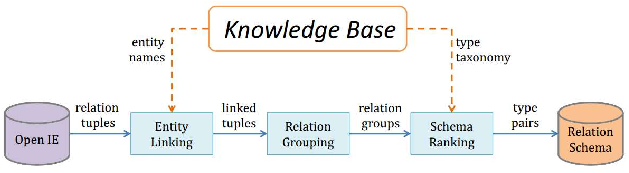
\includegraphics[width=0.9\columnwidth]{figure/tinf/tinf_approach-crop.eps}
    %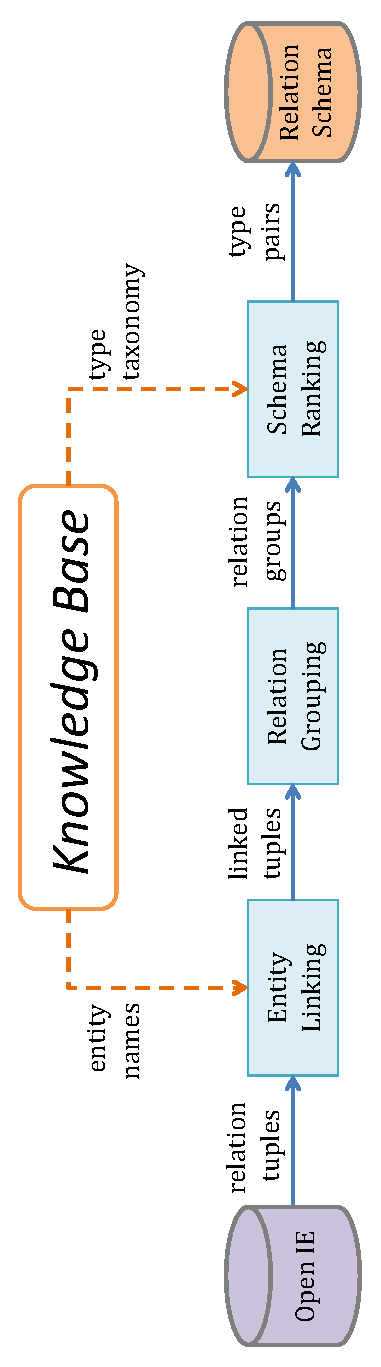
\includegraphics[angle=270,width=\columnwidth]{figure/tinf/system-crop.eps}
    \bicaption{二元关系模式挖掘的流程框图。}{System architecture of type inference of binary relations.}
    \label{fig:tinf-workflow}
\end{figure*}
%\KZ{Redraw this figure as the three boxes in the middle turned out to be
%black in my version of PDF. Also, instead of naming ``ReVerb'' and ``Freebase''
%specifically, use generic terms like ``Open IE'' and ``Taxonomy''. We want
%this system to be general and not tied specifically to ReVerb or Freebase,
%though the actual implementation and eval are on ReVerb and Freebase. These
%we can say in the eval section.}

二元关系模式挖掘的系统架构如\figref{fig:tinf-workflow}所示。
整个系统的输入为开放式信息抽取系统中的所有关系三元组,
经过实体链接、关系分组以及模式排序三个步骤之后,
这些三元组将会转换为一系列排好序的主宾语类型搭配。
每个步骤概括如下,本节将对它们进行具体描述。
%The system takes Open IE relation tuples as the input,
%then performs entity linking, relation grouping and schema ranking
%to translate them into final ranked list of schemas.

% firstly, entity linking (3 sent)
\textbf{(1) 实体链接:}
关系三元组中的参数实体均为字符串形式。
我们通过模糊字符串匹配的方式,将主宾语分别映射到知识库中的不同实体。
%Relation arguments are linked to entities in the knowledge base by
%fuzzy string matching. Each entity in the knowledge base has a unique identifier.

% secondly, relation grouping (2 sent)
\textbf{(2) 关系分组:}
经过链接之后,关系表达形式相近的三元组将聚集在一起,形成一个大的分组。
并且,每一个分组会从内部的不同关系中选择一个,作为整组的代表关系。
%Linked tuples sharing similar relation patterns are grouped together.
%Besides, each group has a representative relation pattern, which is generated from all the patterns within the group.

% thirdly, simultaneously SP (3 sent)
% need to refine at the last sentence.
\textbf{(3) 关系模式排序:}
对分组内的每一个具有链接的关系实例,其主宾语将转换为知识库中对应的类型。
根据不同的类型搭配所覆盖的三元组数量,以及各个类型的宽泛或具体程度,
对所有候选的关系模式进行排序并输出。
%For each linked tuple in one relation group, argument entities are transformed into types drawn from the knowledge base.
%Then this procedure ranks type pairs (schemas) in terms of how much Open IE tuples a type pair can cover and how specific a type concept is.



\subsubsection{实体链接}
\label{sec:tinf-linking}

% 0. what are we going to do ?
% Given a relation tuple, we are going to find representative Freebase entities
% which stand for the arguments.
% 1. Formally definition
在实体链接步骤中,一个关系三元组的主宾语将分别映射到知识库中的实体,
形成带链接的三元组($e_1$, $rel$, $e_2$),并配有对应的链接分值。
%Each entity in Freebase has one or more aliases. The default one is the name of this entity.
%For example, the entity \textit{m.02\_286} has the name ``New York City'' and other aliases
%such as ``The Big Apple'' ``NYC'' and ``Empire City''.
% 4. leverage multiple namees to build an invert index.
由于每一个三元组所具有的信息较少,并没有提供足够的上下文,
因此实体链接过程主要基于主宾语名称以及实体在知识库中名称的模糊匹配。

实体在知识库中存在至多一个标准名称以及多个别名,
例如Freebase中,实体的标准名称和别名分别对应
\textit{type.object.name}以及\textit{common.topic.alias}属性。
我们利用这些属性值构建了从单词指向不同名称的倒排索引,
并进一步生成每个关系参数的候选实体。
% 5. stop word set is used, and use the idf score to weight words.
我们用$alias$表示知识库中的一个名称(或别名),
若将其看做单词的集合(bag-of-words),那么显然单词之间具有不同的重要性。
直观上看,若$alias$中某单词$w$出现在极少数的名称中,那么它对整个名称而言更加重要;
反之类似``of'', ``the'' 等停止词会出现在大多数名称里,那么在模糊匹配的过程中,其权重就很低。
因此我们利用文档频率倒数(Inverted Document Frequency)用于拟合单词$w$的权重:
\begin{equation}
idf(w)=1\ /\log(|\{alias : w \in alias\}|).
\end{equation}
此外,我们直接从知识库的名称中过滤停止词,相当于它们的idf分值为0。
%Besides, stop words are removed from aliases, treating their idf scores as 0.
% 6. matching rule: intersect >= N - 1, weighted overlap score >= threshold
为了衡量关系三元组中的关系参数$arg$与知识库名称$alias$间的模糊匹配程度,
我们计算两者之间的带权重叠分值:
\begin{equation}
overlap(arg, alias) = \frac {\sum\limits_{w \in arg \cap alias} idf(w)} {\sum\limits_{w \in arg \cup alias} idf(w)}.
\end{equation}
对于候选实体$e$,我们分别计算其不同名称与关系参数的模糊匹配分值,
最终选取最高分代表实体$e$与关系参数$arg$的匹配度:
\begin{equation}
sim(e, arg) = \max\limits_{alias \in Alist(e)} overlap(arg, alias).
\end{equation}

% \KQ{TODO: Two Strategies: Just choose the best separately, or FB 2-hop connectable}

为了控制候选实体的质量,
对于由$m$个单词构成的关系参数(停止词忽略不计),
我们仅考虑那些存在至少一个名称具有$m-1$个单词重叠,
同时模糊匹配度高于阈值$\tau$的候选实体。
% we can tune the threshold
% we can use formula to show the weighted score, that is intersect / union, weighed.
% 7. multiple matching, select the one with best wScore.
% 8. tie breaker: count occurrence in freebase relations.
%if there still has a tie, the most popular entity is selected. The popularity of an entity is calculated
%by counting number of relations it has in Freebase.
对于每个关系三元组中的主宾语,我们分别抽取匹配度排名前10的候选实体,用于后续的计算。

对单个关系参数进行匹配计算之后,我们将计算关系三元组
($arg_1$, $rel$, $arg_2$)与实体对($e_1$, $e_2$)之间的联合匹配度。
联合匹配度的定义方式有两种。
第一种匹配方式较为朴素(Naive),仅考虑关系中的两个参数与各自实体的匹配程度,
主宾语实体互相之间并无直接影响:
\begin{equation}
    \label{eqn:naive}
    F(arg_1, e_1, arg_2, e_2, rel) = sim(e_1, arg_1) \cdot sim(e_2, arg_2).
\end{equation}

第二种匹配方式除了考虑$e_1$和$e_2$各自的匹配分数,还考虑到了这两个实体之间存在的联系,
在知识库上体现为连接它们的谓词或谓词序列。
我们以$\vec{w}$表示$rel$的所有单词,
$\vec{p}$表示知识库中连接$e_1$和$e_2$的谓词路径,其长度至多为2。
若实体$e_1$与$e_2$可以通过长度为1的路径相连,
则意味着知识库中存在通过某谓词$p$连接的事实三元组$p(e_1, e_2)$。
类似地,若$e_1$和$e_2$之间通过长度为2的路径相连,
则意味着存在$p_1, p_2$以及中间实体$e'$,
使得事实$p_1(e_1, e')$以及$p_2(e', e_2)$存在于知识库中。
我们利用朴素贝叶斯模型,利用条件概率的形式定义
谓词序列$\vec{p}$与关系$\vec{w}$之间的相关程度:
\begin{equation}
\begin{aligned}
    P(\vec{p}\, |\, \vec{w}) & \approx \prod\nolimits_p P(p\, |\, \vec{w})  \\
                        & \propto \prod\nolimits_p P(p) \prod\nolimits_w P(w\, |\, p).
\end{aligned}
\end{equation}

Yao等人\cite{yao2014information}将知识库谓词序列与关系的对应建模为机器翻译模型,
并根据对齐模型IBM Model 1\cite{brown1993mathematics}学习谓词的先验概率$P(p)$以及
转移概率$P(w|p)$。
基于已有工作的概率模型,给定关系后预测谓词序列的条件概率$P(\vec{p}\, |\, \vec{w})$
便可计算得出。
对于候选实体$e_1$和$e_2$,它们之间的谓词序列与关系$rel$越接近,
则实体链接结果越有可能正确。
因此,我们通过枚举$e_1$和$e_2$之间所有满足长度条件的谓词序列,
计算关系实例与实体对之间的相似度:
\begin{equation}
    \label{eqn:full}
    F(arg_1, e_1, arg_2, e_2, rel) = sim(e_1, arg_1) \cdot
               sim(e_2, arg_2) \cdot
		\sum\nolimits_{\vec{p}} P(\vec{p} | \vec{w}).
\end{equation}

由于条件概率$P(\vec{p} | \vec{w})$的计算涉及到大量连乘,
其数值在不同实体对之间的的差别较为明显,
这也使得其在\eqnref{eqn:full}中具有较高的地位。
而当所有候选实体间的谓词序列与当前关系都不相似的时候,
条件概率的随机波动反而会带来不小的干扰。
因此,我们采用了一种集成(Ensemble)方案:
首先定义条件概率阈值$\rho$,
对于当前关系实例的所有候选实体对,
若其中存在至少一条与关系足够相近的谓词序列,
即满足$P(\vec{p}\, |\, \vec{w}) > \rho$时,
模型使用\eqnref{eqn:full}进行整体匹配度计算,
否则模型退回到\eqnref{eqn:naive},使用朴素的方式寻找最佳实体对。
最后,我们选择分数最高的实体对,作为关系三元组的唯一链接结果。


%\footnote{The popularity of an entity is calculated by counting number of relations it has in the taxonomy.}
%The other strategy (SIM) selects all the $\langle ent1,\ ent2 \rangle$ pairs simultaneously,
%where $ent1$ is reachable from $ent2$ in the taxonomy by 1-hop or 2-hop relation.
%Experimental results on these two strategies are shown in Section 4.


% 9. SUTime is used to map years and datetime.

% check other papers, learn how to introduce FB without too much words.
% 10. discard non-match to guarantee accuracy of linking.
% If one argument fails to link to any entity, the corresponding relation tuple is discarded.
% Ranking Method May Change?
%   use wScore threshold to filter entities
%   then sorting by interLen, then popularity ??? (maybe we can have a try afterwards)
%


%\begin{table}[htbp]
%	\centering
%	\caption{Syntactic Transform Rules}
%	\begin{tabular}{|l|l|}
%		%\toprule
%        \whline
%		Category & Pattern Template \\
%		%\midrule
%        \hline
%        % Continuous Tense & \{$adv_1$\} \textbf{be} \{$adv_2$\} verb:VBG \{text\}
%        %                  & $verb_{lem}$ \{phrase\} \\
%		% Participle Tense & \{$adv_1$\} \textbf{have} \{$adv_2$\} verb:VBN \{text\}
%        %                  & $verb_{lem}$ \{phrase\} \\
%        % Participle + Passive & \{$adv_1$\} \textbf{have} \{$adv_2$\} been \{text\}
%        %                      & is \{text\} \\
%        Continuous Tense & \textbf{be} verb:VBG \{phrase\} \\
%		Participle Tense & \textbf{have} verb:VBN \{text\} \\
%        Future Tense & \textbf{will}/\textbf{shall} verb:VB \{pharse\} \\
%                     & \textbf{be} going to verb:VB \{phrase\} \\
%		%\bottomrule
%        \whline
%	\end{tabular}%
%	\label{tab:synt rules}%
%\end{table}




\subsubsection{关系分组}
% 8 sents.
% 1. group tuples together, give definition
%A relation group consists of linked tuples sharing similar relation patterns,
%along with a representative pattern.
% 2. same & syntactically similar rel. patterns will be in a group, no overlapping.
%Each linked tuple belongs to one unique group.

这个步骤对所有已链接的关系三元组进行聚类,拥有相似关系描述的三元组将归为同一分组。
每个三元组仅存在于唯一一个分组中。

% 3. algorithm: syntactic rules to convert tense,
% mainly focus on 3 tense: will/should/must be, be -ing, participle

%We define syntactically equivalence between two relation patterns, as both of them can be converted
%into the same simple pattern by a list of transformations.
%Every relation pattern in one group is equivalent with each other.
这个步骤的思路是通过语法转换,将复杂的关系描述进行简化。
如果两个不同的关系具有相同的简化形式,那么视为其语义相同,并归为同一分组。
首先考虑到形容词、副词以及情态动词的存在与否,
基本上不会改变一个关系中主宾语实体所属的类型,
因此我们将这些词从关系描述中移除。
此外,大多数关系包含动词,但时态并不一致,
因此我们将所有时态统一为现在时。
此外,关系中的被动语态将会被保留,不做形式转变。
% 4. Create a table, showing the rules to find them.
%The detail of syntactic rules is shown in Table 1.
%\KQ{refer to Liang et al., 2014 to build the rule table, containing continuous, participle, be-the-name-of
%and passive form}
% For example, a --> b
% check liang's 14 paper to learn the representation of tables.
% 5. use stanford parser to tokenize & postag.
% 6. representative relation: present tense
例如经过语法转换之后,下列关系实例将归为同一组:
(X, \textit{resign from}, Y), (X, \textit{had resigned from}, Y)
以及(X, \textit{finally resignd from}, Y)。
最后,每一个分组的代表关系为组内关系的统一简化形式。
如上例所示,三个关系实例属于\textit{``resign from''}组。


\subsubsection{类型搭配排序}
\label{sec:tinf-approach-sort}

给定一个关系分组$r$,这一步骤将生成排好序的主宾语类型对,即该关系的代表性模式。
以二元关系 ``play in'' 举例,理想情况下,生成的结果里会包含模式
$\langle actor,\ film \rangle$以及$\langle pro\_athlete,\ sports\_league \rangle$。

对于带链接的三元组($e_1$, $rel$, $e_2$),
若在知识库中,$e_1$具有类型$t_1$,而$e_2$具有类型$t_2$,
那么该三元组为类型搭配 $\langle t_1,\ t_2 \rangle$ 的一个支持实例。
一个实体有可能从属于多种类型,无论类型宽泛或具体,因此一个三元组可以支持多种类型搭配。
对关系分组$r$中的所有实例进行处理,我们可以得到每一种类型搭配
所对应的支持集合:
\begin{equation}
sup_{r}(\langle t_1, t_2 \rangle) = \{ \langle e_1, e_2 \rangle\ |\ (e_1, t_1) \in IsA,\; (e_2, t_2) \in IsA \}.
\end{equation}

得到所有可能的类型搭配之后,我们可以根据支持集合的大小进行排序。
由于每个实体从属于多种类型,因此显然更加宽泛的类型搭配通常会被排在前列。
但是,对于人类或是机器理解一个自然语言关系,宽泛的关系模式所具有的信息量相对不足,
尤其是当两种类型对具有几乎一致的支持集合时,往往更具体的类型对具有更好的代表性。
例如对于关系 ``\textit{X die in Y}'' ,
在开放式信息抽取和实体链接均不产生错误的情况下,
类型对$\langle person,\ location \rangle$和
$\langle deceased\_person,\ location \rangle$将对应完全一致的支持集合。
后者对关系的描述更加具体,在不丢失支持实例的同时,尽可能缩小主语在知识库中的范围。

由此可见,对候选类型对的排序需要考虑每个类型的相对粒度。
接下来的目标就是提取知识库中类型之间的包含关系,建立更加完整的层次结构。
我们定义所有属于类型$t$的实体为
$cover(t) = \{e\; |\; (e, t) \in IsA\}$。
理想情况中,若$t_1$包含于$t_2$,
那么所有$t_1$中的实体都从属于$t_2$,
即$cover(t_1) \subseteq cover(t_2)$.
这样的包含规则称为 ``{严格类型包含}'' 。
例如在Freebase中,类型\textit{person}所包含的其它类型包括
\textit{actor},\textit{politician}以及\textit{deceased\_person}等。

然而,严格类型包含在知识库中并不多见,
主要原因是知识库的类型定义和人类对自然界的归纳存在一定差别,
以Freebase中的\textit{award\_winner}为例,
类型中绝大多数实体都为自然人,但依然包含少量的组织实体在内。
基于严格类型包含的规则,
\textit{award\_winner}与\textit{person}之间毫无包含关系,
但事实上,考虑到非自然人实体仅存在极少数,
两个类别之间在很大程度上依然构成从属关系。
另一方面,由于实体的类型涉及到人工标记,一旦出现类型标记错误,
就有可能导致类型之间无法满足严格包含条件。


为了能更好地建立类型层次关系,我们使用一种更加松弛的类型包含定义方式。
具体而言,若$t_1$中足够数量的实体从属于$t_2$,那么就认为包含关系成立。
因此,我们定义$t_1$包含于$t_2$的度,即对应实体包含的比例:
\begin{equation}
deg(t_1 \subseteq t_2) = \frac{\left|cover(t_1) \cap cover(t_2)\right|} {\left|cover(t_1)\right|}.
\end{equation}
%$deg(Supp_1\subseteq Supp_2)=\left|Supp_1 \cap Supp_2\right| / \left|Supp_1\right|$.
若$deg(t_1 \subseteq t_2) > \epsilon$,
则$t_1$包含于$t_2$。
阈值$\epsilon$表示松弛程度,若$\epsilon=1$,则松弛包含退化为严格包含。
若$\epsilon$太小,那么类型之间将具有非常丰富的层次关系,
但其有效性则会下降。
最后,遍历知识库中所有的类型,我们就可以得到特定松弛程度下的类型层次图。
%\figref{fig:tinf-taxonomy}展示了Freebase中的一部分类型之间的层次关系,
%用不同样式的边表示不同松弛程度的包含。
%TODO: taxonomy弄一个好一点的图,可以撑1/3页呢。

随着类型层次关系建立完毕,我们就可以定义不同类型搭配之间的包含关系。
若类型对$\langle t_1,\ t_2\rangle$被另一个类型对
$\langle t_3,\ t_4\rangle$,则意味着以下条件之一成立:
i) $t_1 \subseteq t_3$,$t_2 \subseteq t_4$;
ii) $t_1 \subseteq t_3$,$t_2 = t_4$;
iii) $t_2 \subseteq t_4$,$t_1 = t_3$。
最终的类型对排名体现为支持集合大小和类型对包含关系的共同作用。
以支持集合降序排列为基础,
若类型对$tp=\langle t_1, t_2 \rangle$包含于另一个类型对$tp'$,
且各自的支持集合大小($|sup_{r}(tp)|$)几乎一致,
那么$tp'$将排在$tp$之前。
我们同样可以根据重叠关系实例的覆盖程度,
来定义两个支持集合是否几乎一致:
\begin{equation}
\frac{\left|sup_{r}(tp)\right|-\left|sup_{r}(tp')\right|} {max(\left|sup_{r}(tp)\right|,\ \left|sup_{r}(tp')\right|)} < \lambda,
\end{equation}
其中$\lambda$为判断集合中的元素是否一致的阈值。

